\documentclass[a4paper, 12pt]{book}

\usepackage[utf8]{inputenc}
\usepackage{blindtext}
\usepackage{graphicx}
\usepackage{pgfplotstable}
\usepackage{booktabs}
\usepackage{filecontents}
\usepackage{longtable}
\usepackage[T1]{fontenc}
\usepackage[backend=biber]{biblatex}
\addbibresource{references.bib}
\usepackage[skip=5pt plus1pt, indent=0pt]{parskip}

\graphicspath{ {./images/}{./troubleshooting/crumb-structures/} }


\title{%
  The Sourdough Framework\\
  \large How to master making bread at home\\
  \small - the bread code community book -}

\author{Hendrik Kleinwächter}
\date{\today}

\begin{document}

\begin{titlepage}
\maketitle
\end{titlepage}


\frontmatter

\tableofcontents

\chapter{Foreword}
Still need someone to write a foreword

\chapter{Preface}
If there is one food Germany is known for, it is probably bread.
There are thousands of varieties in Germany,
and making it has been an integral part of our culture.

My bread journey began during childhood. My mother, being a parent
of 3, would always use Saturdays to bake a delicious loaf for the family.
It was a white fluffy sandwich bread, and she made it within one to two hours using store-bought yeast.
Being a bit more experienced, I now realize it's
ideal to wait a little while before cutting into your bread, but back then,
we kids couldn't wait. Mom would cut for us a few slices straight from the oven, and we would
immediately proceed to pour butter or jam on each slice. Within minutes, 1kg of
flour would be consumed. Bread became an integral part of my weekly food.

I was lucky that my parents could afford a yearly ski trip to
Alto Adige in northern Italy. In the small town called Valdaora, we
would try new restaurants every year, yet always end up in our favorite
pizza place. The pizzas there were incredible. The dough
alone was so tasty that we would order just the bread with a
bit of olive oil and salt.

Of course, my question would always be, ``Mom, can we make this at home, too, please?''
So over the years, we became friends with the owners and would receive
more and more clues as how to make the perfect pizza dough. There
are no secret ingredients inside. It's just flour, water, salt, and a bit of yeast.
How can such a simple combination of ingredients create such an incredibly delicious
pizza dough? My parents, being creatures of habit, would return every year with us,
and every year, my interest would grow. At home, Mom and I attempted to replicate
the recipe. We tried baking on a stone and on a steel. We tried adding oil to the dough and herbs
to the pizza sauce. We fell into an endless cycle of experiments. However, we never managed
to get close to the experience we had while on vacation.

Some years passed, and I eventually began my studies in the small German city of Göttingen.
For the first time, I was faced with shopping for my own bread. It was never
on my mind to actually start baking it for myself. I would just buy 
a good loaf while shopping at the supermarket. My favorite variety
was a Schwarzbrot, Korn an Korn. It’s a very dark and hearty rye bread
with added berries and sunflower seeds. Being a little naive,
I'd never before examined the packaging of what I was buying. One day, that
changed.

I looked at the label and was shocked. The seemingly
healthy bread consisted of so many other things aside from flour and water.
The black color was not coming from the flour, but from caramelized sugar.
The packaging stated it was a sourdough bread, but then why was there additional yeast?
I thought that if it was really sourdough, it shouldn't require additional yeast, and I
soon realized that something was wrong with the bread I was buying.
I proceeded to check the other supermarket breads, only to discover that they, too,
contained ingredients I'd never heard of. That was the day I lost trust
in supermarket bread.

At home, I decided to research the proper way to make bread, and much to my surprise,
I learned that the recipes for making pizza and bread were actually quite similar, yet
there were also diffferences. For example, some recipes would call for fresh yeast, while
others would call for dry. Deep diving into various online forums and all their many
discussions, I became even more confused.

I tried using different flours and different brands, all in both organic and non-organic varieties.
I realized then that I knew nothing about making bread. Recipes would often contradict each other,
leaving me further confused. They seemed like little more than a collection of apparently random
steps to follow. The baking instructions and temperatures were all different, too.

Meanwhile, having completed my studies, I started work as an engineer.
We engineers are faced with many challenges. The compiler or runtime is
always screaming at you with errors, and it's your job to figure out how to fix them.
It can take hours, sometimes days just to fix a simple problem. If you want
to become a software engineer, you have to develop a certain ``never-give-up'' attitude.

Frequently when writing code, a set of pre-made routines are required. These routines have been
written by other engineers and can then be used to ship code faster.
This pre-written code is commonly known as {\it a framework}. In many cases,
these frameworks are not built by a single person but by engineers from all around the world,
each of whom can help by improving and changing the source code. Frameworks have made many successful
businesses possible.

In most cases, frameworks do exactly what they claim they do. However,
sometimes you are faced with issues you don't understand. In 99.95 percent
of all software bugs, the developer is the issue. Sometimes, however, the framework has a
bug. That is when the developer must dig deeper to see the what and the why behind what the
framework is doing. You will need to read other engineer's source code, and you will be forced
to understand {\it why} things are happening.

Being unhappy with what I was baking, my engineering mindset took over and I had
to do my own deep dive to understand what was going on. Much to my surprise, however,
none of the recipes I'd encountered would tell me {\it why} I should use amount X
of water and amount Y of flour, or {\it why} exactly I should use fresh yeast over dry yeast. Why
should I slap my dough while kneading it on the counter? Why is a standmixer
better than kneading by hand?  Why should I let the dough sit for this long?
Why is steaming the dough during baking important? Do I really need to
get myself an expensive dutch oven to bake bread?

The problem compounded when I started reading about sourdough. It all sounded like black
magic. Why were some sourdoughs made from fruits, while others were made from flour?
Why should one recipe use wheat while another used rye or spelt? How often should the
sourdough be fed? The questions I had then could have filled 20 pages. I was confused,
but became even more determined to learn how decent bread should be made at home.

The feedback I received from friends helped me to improve with each
iteration of homemade bread. Compared to coding, where you sometimes have to wait months
for this feedback, bread making is much more direct. Plus, you can eat your successes
(and failures!) And, much to my surprise, even those failures started tasting better than
most store-bought breads. Eating a homemade bread that takes you hours to make allows you
to develop a different relationship with your food, and baking bread from scratch with my
bare hands was a welcome change after hours of working on the computer.

I continued learning about the process of fermentation and various techniques of bread making.
I approached the topic of sourdough in a manner similar to software, and after years of
researching and documenting my progress, I decided it was time to share that progress with the
world.

When working on open source projects, it is important to see their history and how the source
code changes over time. This way, you can easily jump back to previous versions. This was
the perfect tool for documenting my recipes, because they, too, would change with each
subsequent iteration. Much to my surprise, my open source work on sourdough was appreciated
by other engineers, and the project became popular on the website GitHub, originally built to
share open source software.

Now, when baking great bread, you also need to learn certain techniques. I figured it would be
easier to share these techniques in video form. Thus, my YouTube channel was born. I chose
the name {\it The Bread Code} to capture my engineering-oriented approach to bread. It took some
time to get right, but after choosing more engaging thumbnails and titles for
the videos I made, the channel started gaining viewers.

Now, three years later, I dedicate two days each week to follow my bread baking passion, while
the other three days I continue to work as a software engineer, writing code on a day-to-day
basis.

My bread days fill me with both joy and passion. To me, there is nothing better than seeing
how many people have made amazing bread thanks to my tips and explanations. The community has
continued to grow, spawning many interesting discussions and ideas surrounding the topic of
bread making. There is always something new to learn, and I feel that even now I am just barely
scratching the surface with what I know and teach. Would you ever have imagined that fruit
flies are like bees and are part of the wild yeast's success story? I made a video where
I tried to cultivate wild yeast spores coming from fruit flies in order
to bake bread. It worked; the bread turned out amazing and even tasted good! These kinds of
experiments spark my natural interest. Conducting them and seeing how other people share in my
interest makes me incredibly happy.

The problem with running a YouTube channel is that all the information
you see is filtered and then provided to you through an algorithm. I am concerned
with how algorithms are shaping modern information, because they tend to
put users into certain categories where they will then only see news related to
those same fixed categories. A key metric determining visibility of your channel is how many
people have clicked on a video after it's been shown, and the content you create
is not even shown to every subscriber of your channel. If the algorithm determines the video
is not engaging enough, your content starts to decay in YouTube's nirvana. Even if your video
goes viral, the algorithm will stop showing it once engagement rates with new users goes down,
and older videos fade over time as the decay punishment factor increases. I know, because
I have developed similar algorithms myself as a software engineer.

I've since decided to take some time off from the algorithm cycle to work on something more
long term and meaningful. My mission has always been to share my knowledge with as many people
in the world as possible. That's also why my content has been provided in English rather than
German. After discussing with members of the community, I figured that writing a book could
help me achieve that goal. Most of the books that exist today are collections of recipes. My
idea, however, is to provide you with a deeper foundation of knowledge that you can use to
follow other recipes.

In software terms, this would be a {\it bread framework}.

It is my goal for this book to help everyone facing issues with flour, fermentation, baking,
and more. It should provide a detailed understanding as to why certain steps are necessary
and how to adapt then when things go wrong while making bread.

It is my desire for this knowledge to be accessible to everyone around the world, regardless
of budget, and as such, do not want to charge for the book. That's why I've decided to make
it open source and have asked the community to support my work financially via my ko-fi page
(https://ko-fi.com/thebreadcode). The community's feedback has been amazing so far, and
I've already raised much more money than initially expected.

The first version of the book will only be available digitally---this way, everyone can read
it---though there might also be a hardcover version in the future, depending on how well received
and appreciated it is by bakers around the world. The hardcover version will, of course, cost a
bit of money, but the digital version will remain free.

In this book, I will try to be as scientific as possible. I in no way claim, however, that
it will itself be a work of science. I have conducted several experiments that I will write
about here, but to truly call this science, you would probably need to repeat the same experiment
a thousand times in a lab environment, which I have not done. I will do my best, however, to provide
scientific references where possible and to clearly distinguish between facts and personal opinion.

I hope you have fun reading this and that you learn more about the fascinating world of bread
making, and it is my sincere wish that this work provides you with the solid toolchain that I wish
I'd had access to when starting my own journey with bread.

Thank you.
Hendrik

\chapter{Acknowledgements}
This book would not have been possible without your help.

With all your donations I have been able to take time off from my job and
focus on this project.

Furthermore many of you have contributed and improved the
instructions, fixed spelling mistakes and/or provided
feedback on the content. Each of you has made this book
better.

By providing this book free of charge,
we can enable more people around the world to bake delicious sourdough
bread at home.

Thank you very much for your support!\\

\begin{filecontents}{supporters.csv}
  \end{filecontents}

  {\large Big shout-out to all the initial supporters:}

  \pgfplotstableset{
  begin table=\begin{longtable},
  end table=\end{longtable},
  }

  \pgfplotstabletypeset[col sep=comma,
  header=true,
  columns={Name},
  columns/Name/.style={column type=l,string type},
  every head row/.style={before row=\toprule, after row=\midrule\endhead},
  every last row/.style={after row=\bottomrule}
  ]{supporters.csv}


\mainmatter

\chapter{The history of sourdough}
\section{Sourdough bread in ancient times}
\section{How modern bread is made}
\section{Sourdough in modern times}

\chapter{How sourdough works}
\section{Enzymatic reactions}
\section{Yeast}
\section{Lactic acid bacteria}
\section{Acetic acid bacteria}

\chapter{Making a sourdough starter}
\section{Baker's math}
\section{The process of making a starter}
\section{How flour is fermented}
\section{Determining starter readiness}
\section{Maintenance}
\section{Longterm starter storage}

\chapter{Sourdough starter types}
\section{The regular starter}
\section{Stiff starter}
\section{Liquid starter}
\section{Lievito madre}

\chapter{Flour types}
\section{Wheat like}
\section{Non gluten binding}
\section{Gluten free}
\section{Blending flours}

\chapter{Bread types}
\section{Wheat bread basics}
\section{Non wheat bread basics}
\section{The simplest way to make bread}

\chapter{Wheat sourdough}
\section{The process}
\section{Readying your starter}
\section{Ingredients}
\section{Hydration}
\section{Autolyse}
\section{Fermentolyse}
\section{Dough strength}
\section{Controlling fermentation}
\section{Optional Preshaping}
\section{Shaping}
\section{Proofing}

\chapter{Non wheat bread basics}
\section{Ingredients}
\section{Managing acidity}
\section{To shape or not to shape}
\section{Proofing}

\chapter{Baking}
\section{The role of steam}
\section{Temperature}
\section{Home oven setup}
\section{Dutch ovens}

\chapter{Storing bread}
\section{Fridge}
\section{Room temperature}
\section{Frozen}

\chapter{Troubleshooting}

\section{Debugging your crumb structure}
The crumb structure of your bread provides insights on how well
your fermentation process has gone. You can also spot common flaws
of improper technique. This chapter will provide you with information
that you can use to debug your baking process.

\subsection{Perfect fermentation}

\begin{figure}
  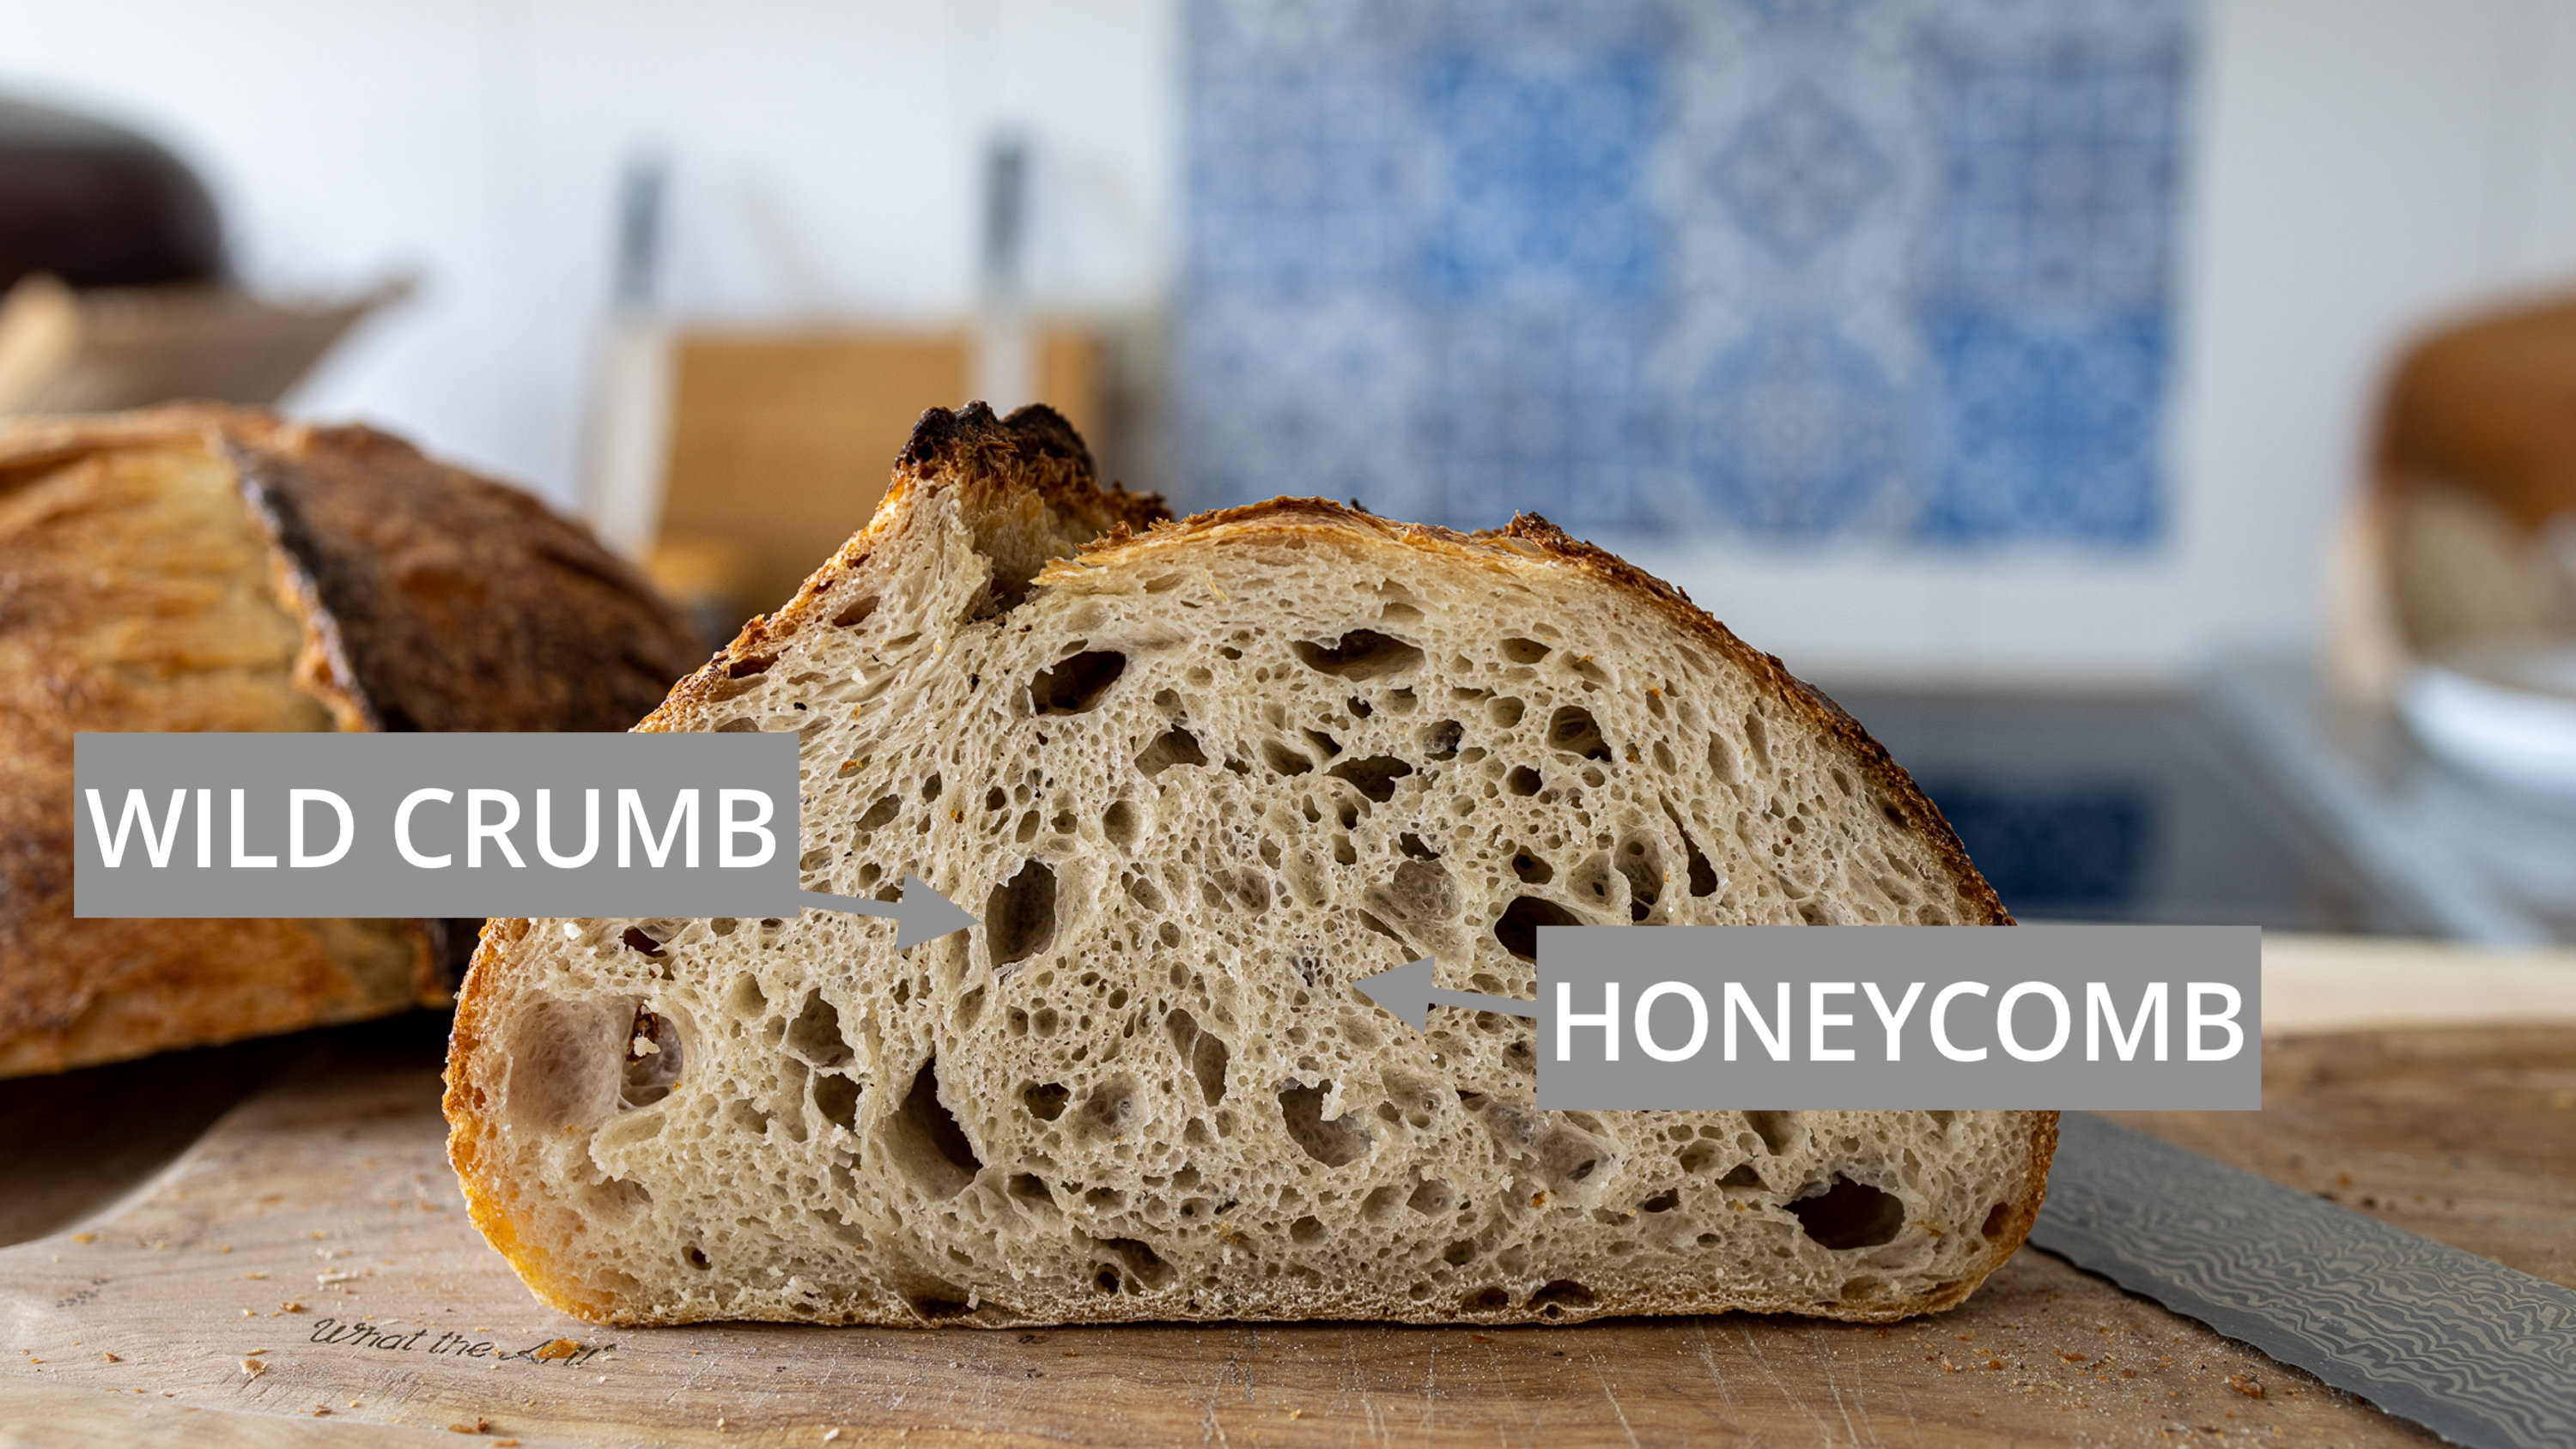
\includegraphics[width=\textwidth]{open-crumb}
  \caption{The bread has a somewhat open crumb with areas
  featuring a honeycomb structure.}
  \label{fig:open-crumb}
\end{figure}

Of course the perfect fermentation is debatable and highly subjective. To
me the perfect sourdough bread features a crisp crust paired with a fluffy
somewhat open crumb. This is the perfect balance of different consistencies
when you take a bite.

Some people are chasers of a very open crumb, meaning you have large pockets
of air (alveoli). It's subjective whether that's the style of bread that you like,
however to achieve it you need to ferment your bread dough perfectly on point.
It takes a lot of skill both in terms of mastering fermentation and technique
to achieve a crumb structure like that.

Me personally I like a bread like that, just with a slightly less wild crumb.
The style of crumb I like is called the {\it honeycomb crumb}. It's not too open, but
just enough open to make the bread very fluffy. To achieve the previously mentioned open crumb you
have to touch your dough as little as possible. The more you interact with your
dough the more you are degassing your dough. Excess touching of the dough
results in the dough's alveoli merging together. The crumb will not be as open.
That's why achieving such a crumb works best if you only ferment
one dough at the same time. Normally if you have to preshape your dough,
you will automatically degas your dough a little bit during the rounding process.
If you skip this step and directly shape your dough you will achieve a more open crumb.
A good rule of thumb is to not touch your dough for at least 1-2 hours before shaping,
to achieve an as open crumb as possible.

\begin{figure}
  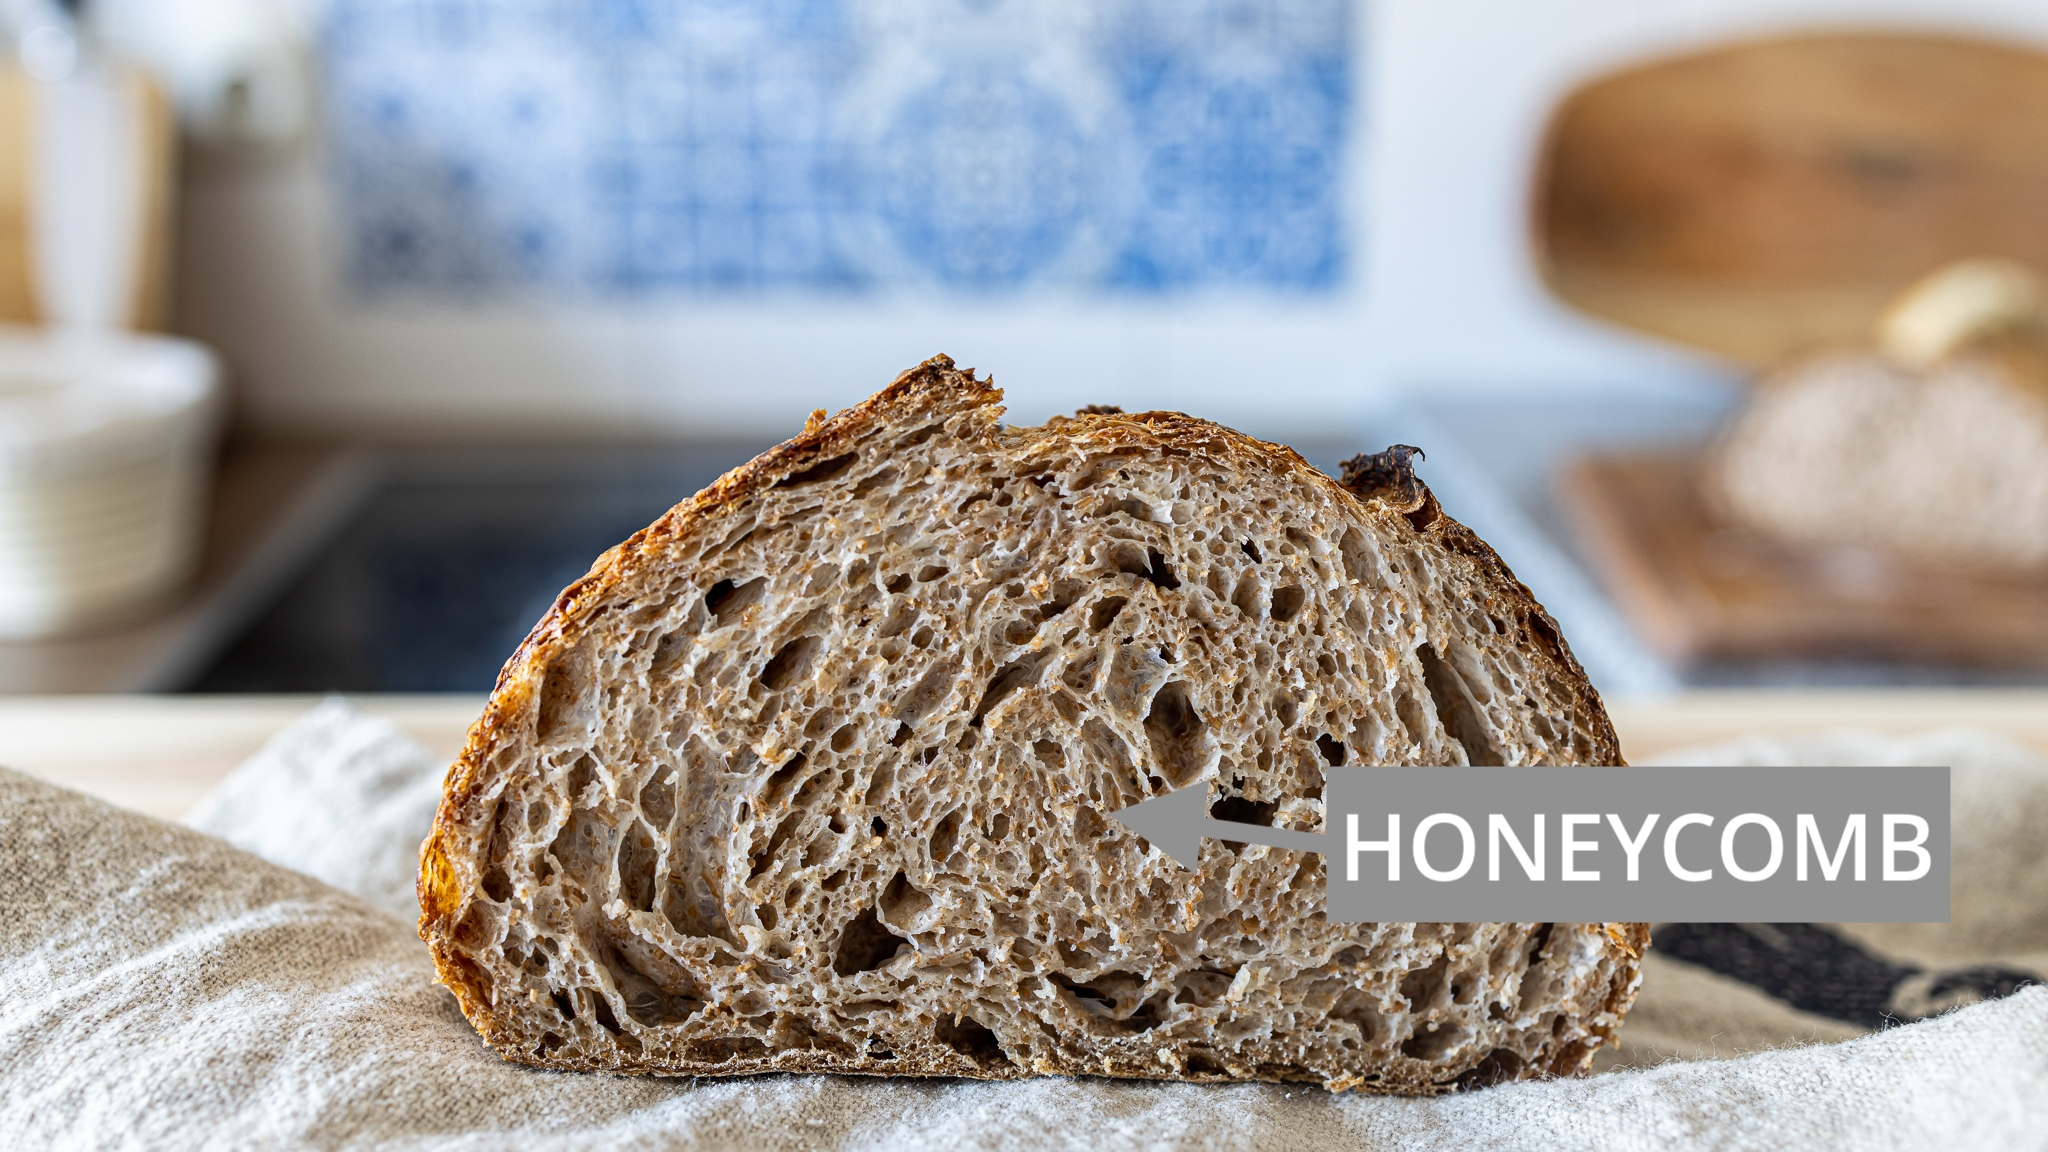
\includegraphics[width=\textwidth]{honeycomb}
  \caption{A whole wheat sourdough with an almost exclusive honeycomb crumb structure.}
  \label{fig:honeycomb}
\end{figure}


Now this is problematic when you want to
make multiple breads at the same time. Preshaping is essential as you are required
to divide your large bulk dough into smaller chunks. Without the preshaping
process you would end up with many non-uniform bread doughs. This technique is
also used when making ciabattas. They are typically not shaped. You only cut the
bulk dough into smaller pieces, trying to work the dough as little as possible.
With preshaping you will converge your dough's alveoli into more of a honeycomb structure,
as large pockets of air will slightly converge. Similarly to the open crumb structure
you also have to nail the fermentation process perfectly to achieve this crumb.
A too long fermentation will result in gas leaking out of your dough while baking.
The honeycomb's won't be able to retain the gas. If you ferment for too short,
there is not enough gas to inflate the structures. To me this is the perfect
style of crumb. As someone who appreciates jam, no jam will fall through a slice
of this bread compared to an open crumb.

\subsection{Overfermented}

\begin{figure}
  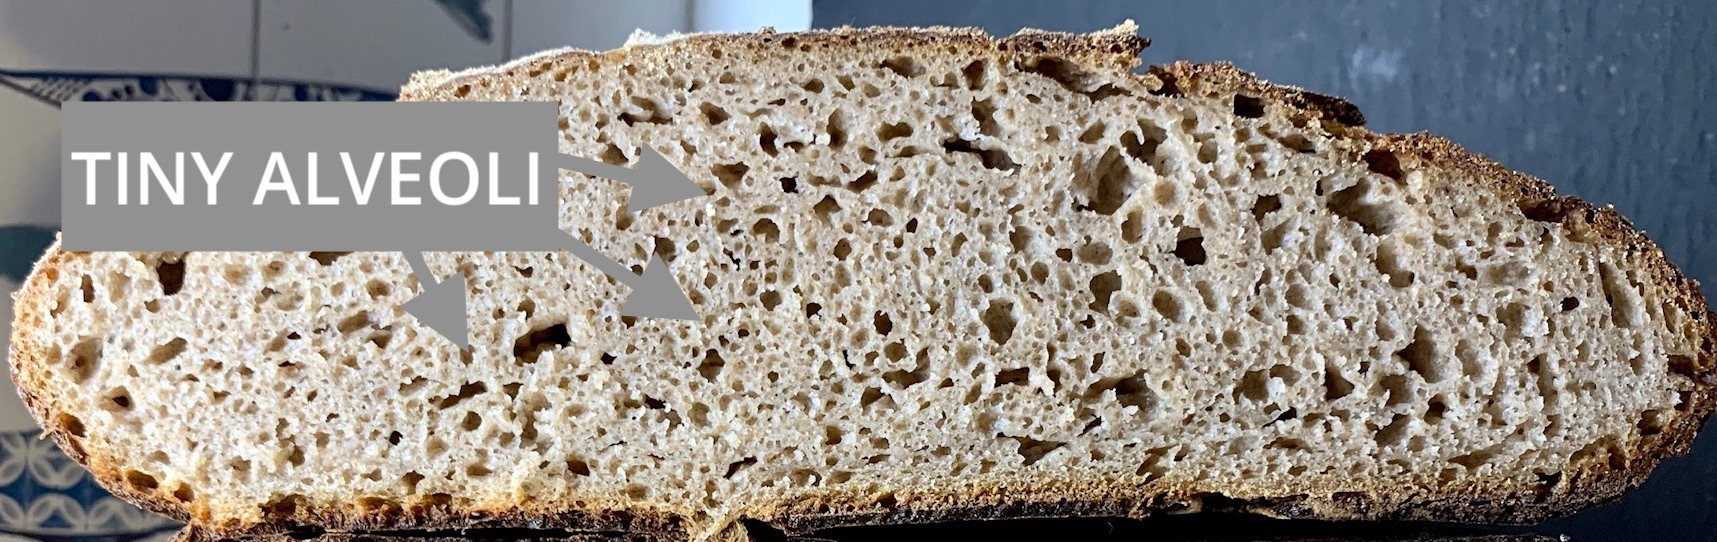
\includegraphics[width=\textwidth]{fermented-too-long}
  \caption{A relatively flat dough that has many tiny pockets of air.}
  \label{fig:fermented-too-long}
\end{figure}

When fermenting your dough for too long over time the protease enzyme starts to
break down the gluten of your flour. Furthermore the bacteria consumes the gluten
in a process called {\it proteolysis} \cite{raffaella+di+cagno}.
Bakers also refer to this process as {\it gluten rot}.
The gluten that normally is normally trapping the CO2 created
by the fermentation process of your microorganisms can no longer stay inside of
the dough. It disperses outward resulting in smaller alveoli in your crumb.
The bread itself tends to be very flat in the oven. Bakers often refer
to this style of bread as a {\it pancake}. The oven spring can be compared
to bread doughs made out of low gluten flour like Einkorn.

Your bread will feature a lot of acidity, a really strong distinctive tang. From
a taste perspective it might be a little bit too sour. From my own tests with family and
friends (n=15-20) I can say that this style of bread is typically
not as appreciated. However, me personally I really like the hearty strong taste.
It is excellent in combination with something
sweet or a soup.  From a consistency perspective it is no longer as fluffy as it could be.
The crumb might also taste a little bit gummy. That's because it has been broken down a lot
by the bacteria. Furthermore this style of bread has a significantly lower amount of gluten \cite{raffaella+di+cagno}
and is no longer comparable to raw flour, it's a fully fermented product.
You can compare it with a blue cheese that is almost lactose free.

When trying to work with the dough you will notice that suddenly the dough feels
very sticky. You can no longer properly shape and work the dough. When trying to
remove the dough from a banneton the dough flattens out very much. Furthermore
in many cases your dough might stick to the banneton. When beginning with baking
I would use a lot of rice flour in my banneton to dry out the surface of the dough a lot.
This way the dough wouldn't stick, despite being over fermented. However as it
turns out the stickiness issue has been my lack of understanding the fermentation
process. Now I never use rice-flour, except when trying to apply decorative scorings.
Properly managing fermentation results in a dough that is not sticky.

If you are noticing during a stretch and fold, or during shaping that your dough
is suddenly overly sticky, then the best option is to use a loaf pan. Simply take
your dough and toss it into a loaf pan. Wait until the dough mixture has increased
in size a bit again and then bake it. You will have a very well tasting sourdough
bread. If it's a bit too sour, you can just bake your dough for a longer period
of time to boil some of the acidity during the baking process. You can also use
your dough to setup a new starter and try again tomorrow. Lastly if you are hungry
you can simply pour some of your dough directly into a heated pan with a bit of
oil. You will be making delicious sourdough flat breads.

To fix issues related to overfermentation you need to stop the fermentation process
earlier. What I like to do is to extract a small fermentation probe from my dough.
Depending on the volume increase of this probe I can mostly judge when my fermentation
is finished. Try to start with a 25 percent volume increase of your main dough or sample.
Depending on how much gluten your flour has, you can ferment for a longer period of time.
With a strong flour featuring a 14-15 percent protein you should be able to safely
ferment until a 100 percent size increase. This however also happens on your
sourdough starter's composition of yeast and bacteria. The more bacterial fermentation
the faster your dough structure breaks down. Frequent feedings of your sourdough
starter will improve the yeast activity. Furthermore a stiff sourdough starter
might be a good solution too. The enhanced yeast activity will result in a more fluffy
dough with less bacterial activity. A better yeast activity also will result
in less acidity in your final bread. If you are a chaser of a very strong tangy
flavor profile then a stronger flour with more gluten will help.


\subsection{Underfermented}

\begin{figure}
  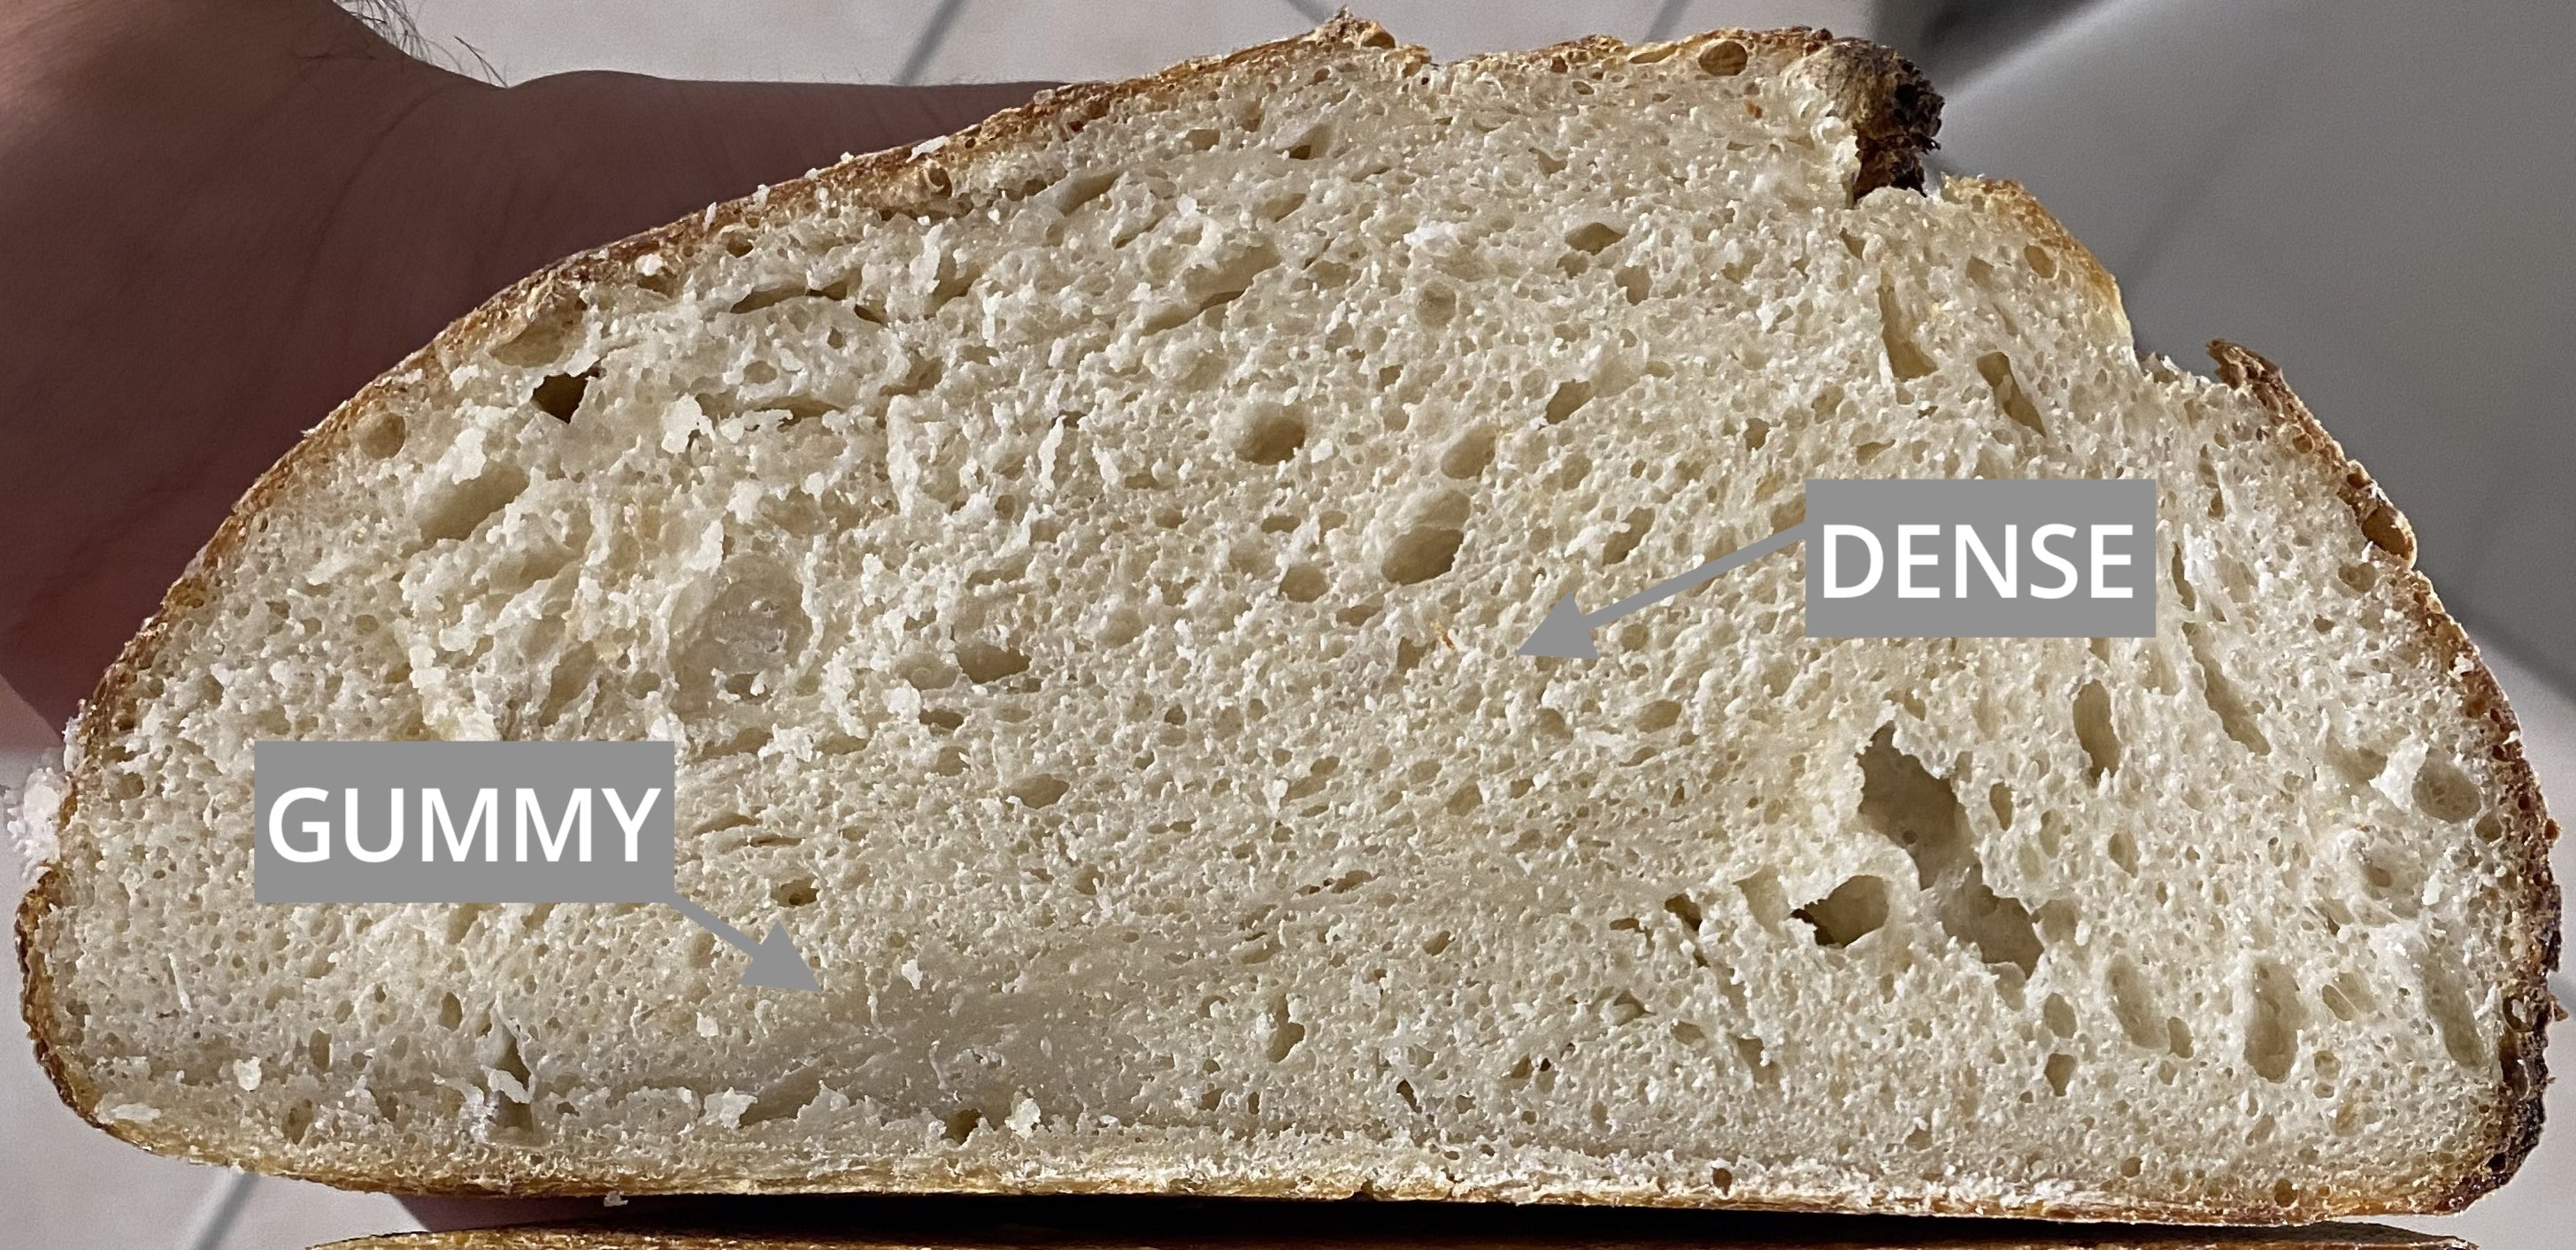
\includegraphics[width=\textwidth]{fermented-too-short-underbaked}
  \caption{A dense dough featuring a gummy not fully gelatinized area.
  The picture has been provided by Midori from our community discord server.}
  \label{fig:fermented-too-short-underbaked}
\end{figure}

This defect is also commonly referred to as {\it underproofed}. However underproofed
is not a good term as it only refers to having a too short period of time in the final
proofing stage of the bread making process. If you were to directly bake your bread
after a successful bulk fermentation stage you would not achieve this defect.
Proofing will make your dough a bit more extensible and allows your sourdough
to inflate the dough a bit more. When faced with an underfermented bread you
already did something wrong during the bulk fermentation stage, or maybe also
even before that with your sourdough starter.

A typical underfermented dough has very large pockets of air and is partially
wet and gummy in some areas of the dough. The large pockets can be compared
to making a non-leavened wheat or corn tortilla. As you bake the dough in your pan
the water slowly starts to evaporate. The gas is trapped in the structure of the dough
and will create pockets. In case of a tortilla this is the desired behavior.
But when you observe this process in a larger dough you will create several
super alveoli. The water evaporates and the first alveoli form. Then at some point
the starch starts to gelatinize and becomes solid. This happens first inside of the pockets
as the interior heats up faster compared to the rest of the dough. Once all the starch
has gelatinized the alveoli holds its shape and no longer expands. During this
process other parts of the bread dough are pushed outwards. That's why an underfermented
dough sometimes even features an ear during the baking process. This
is also commonly referred to as a {\it fool's crumb}. You are excited about an ear which
can be quite hard to achieve. Plus you might think you finally created some big pockets
of air in your crumb. But in reality you fermented for a too short period
of time.

\begin{figure}
  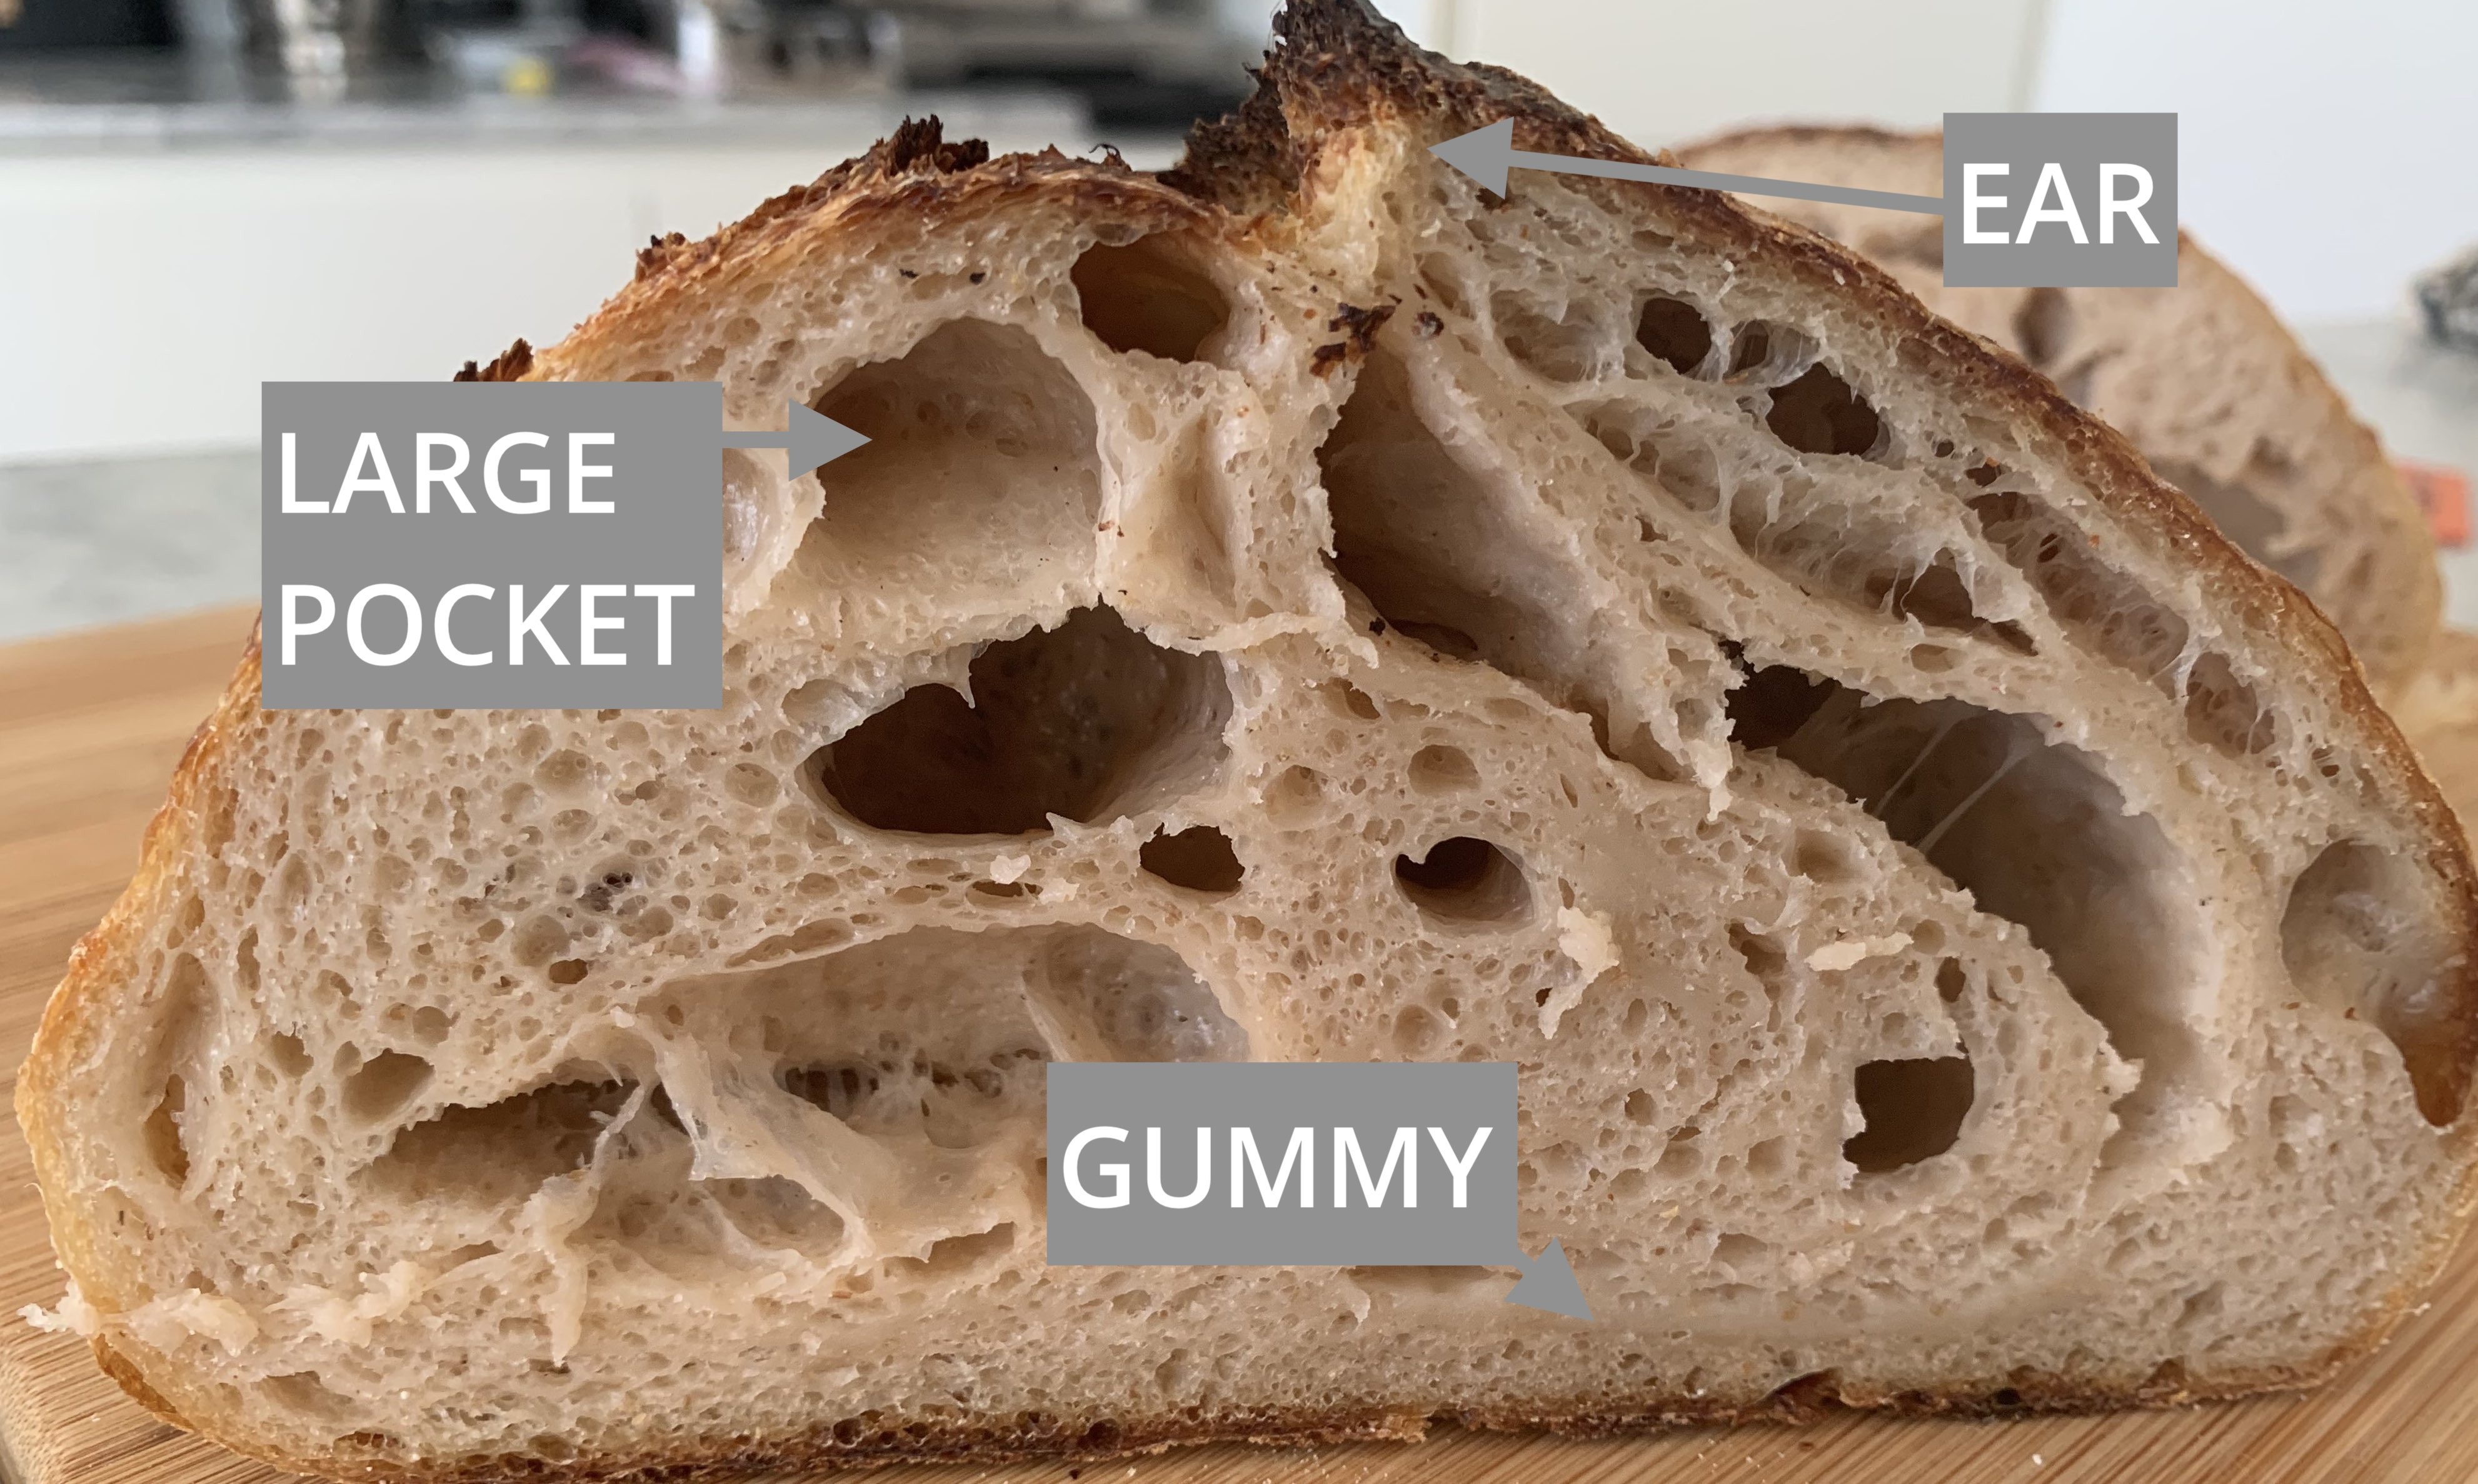
\includegraphics[width=\textwidth]{fools-crumb}
  \caption{A typical example of a fool's crumb featuring an ear and several overly
  large alveoli. The picture has been provided by Rochelle from our
  community discord server.}
  \label{fools-crumb}
\end{figure}

In a properly fermented dough the alveoli help with the heat transfer throughout the dough.
From within the tiny many fermentation induced pockets the starch gelatinizes. With
an underfermented dough this heat transfer does not properly work. Because of that
you sometimes have areas which look like raw dough. Bakers refer to this as a very
gummy structure sometimes. Baking your dough for a longer period of time would also properly
gelatinize the starch in these areas. However, then other parts of your bread
might be baked too long.

To fix issues related to underfermentation you simply have to ferment your dough
for a longer period of time. Now there is an upper limit to fermentation time
as your flour breaks down the moment it is in contact with water. That's why it
might be a good idea to simply speed up your fermentation process. As a rough
figure, I try to aim for a bulk fermentation time of around 8-12 hours typically.
To achieve that you can try to make your sourdough starter more active.  This can be done
by feeding your starter daily over several days. Use the same ratio as you would
do for your main bread dough. Assuming you use 20 percent starter calculated on the flour,
use a 1:5:5 ratio to feed your starter. That would be 10 grams of existing starter,
50 grams of flour, 50 grams of water for instance. To boost your yeast even more you can
consider making a stiff sourdough starter. The stiff sourdough starter will
boost your yeast activity. The bacteria produces mostly acid. The more acidity
is piled up, the less active your yeast is. The stiff sourdough starter
enables you to start your dough's fermentation with yeast dominated activity.


\subsection{Not enough dough strength}

\begin{figure}
  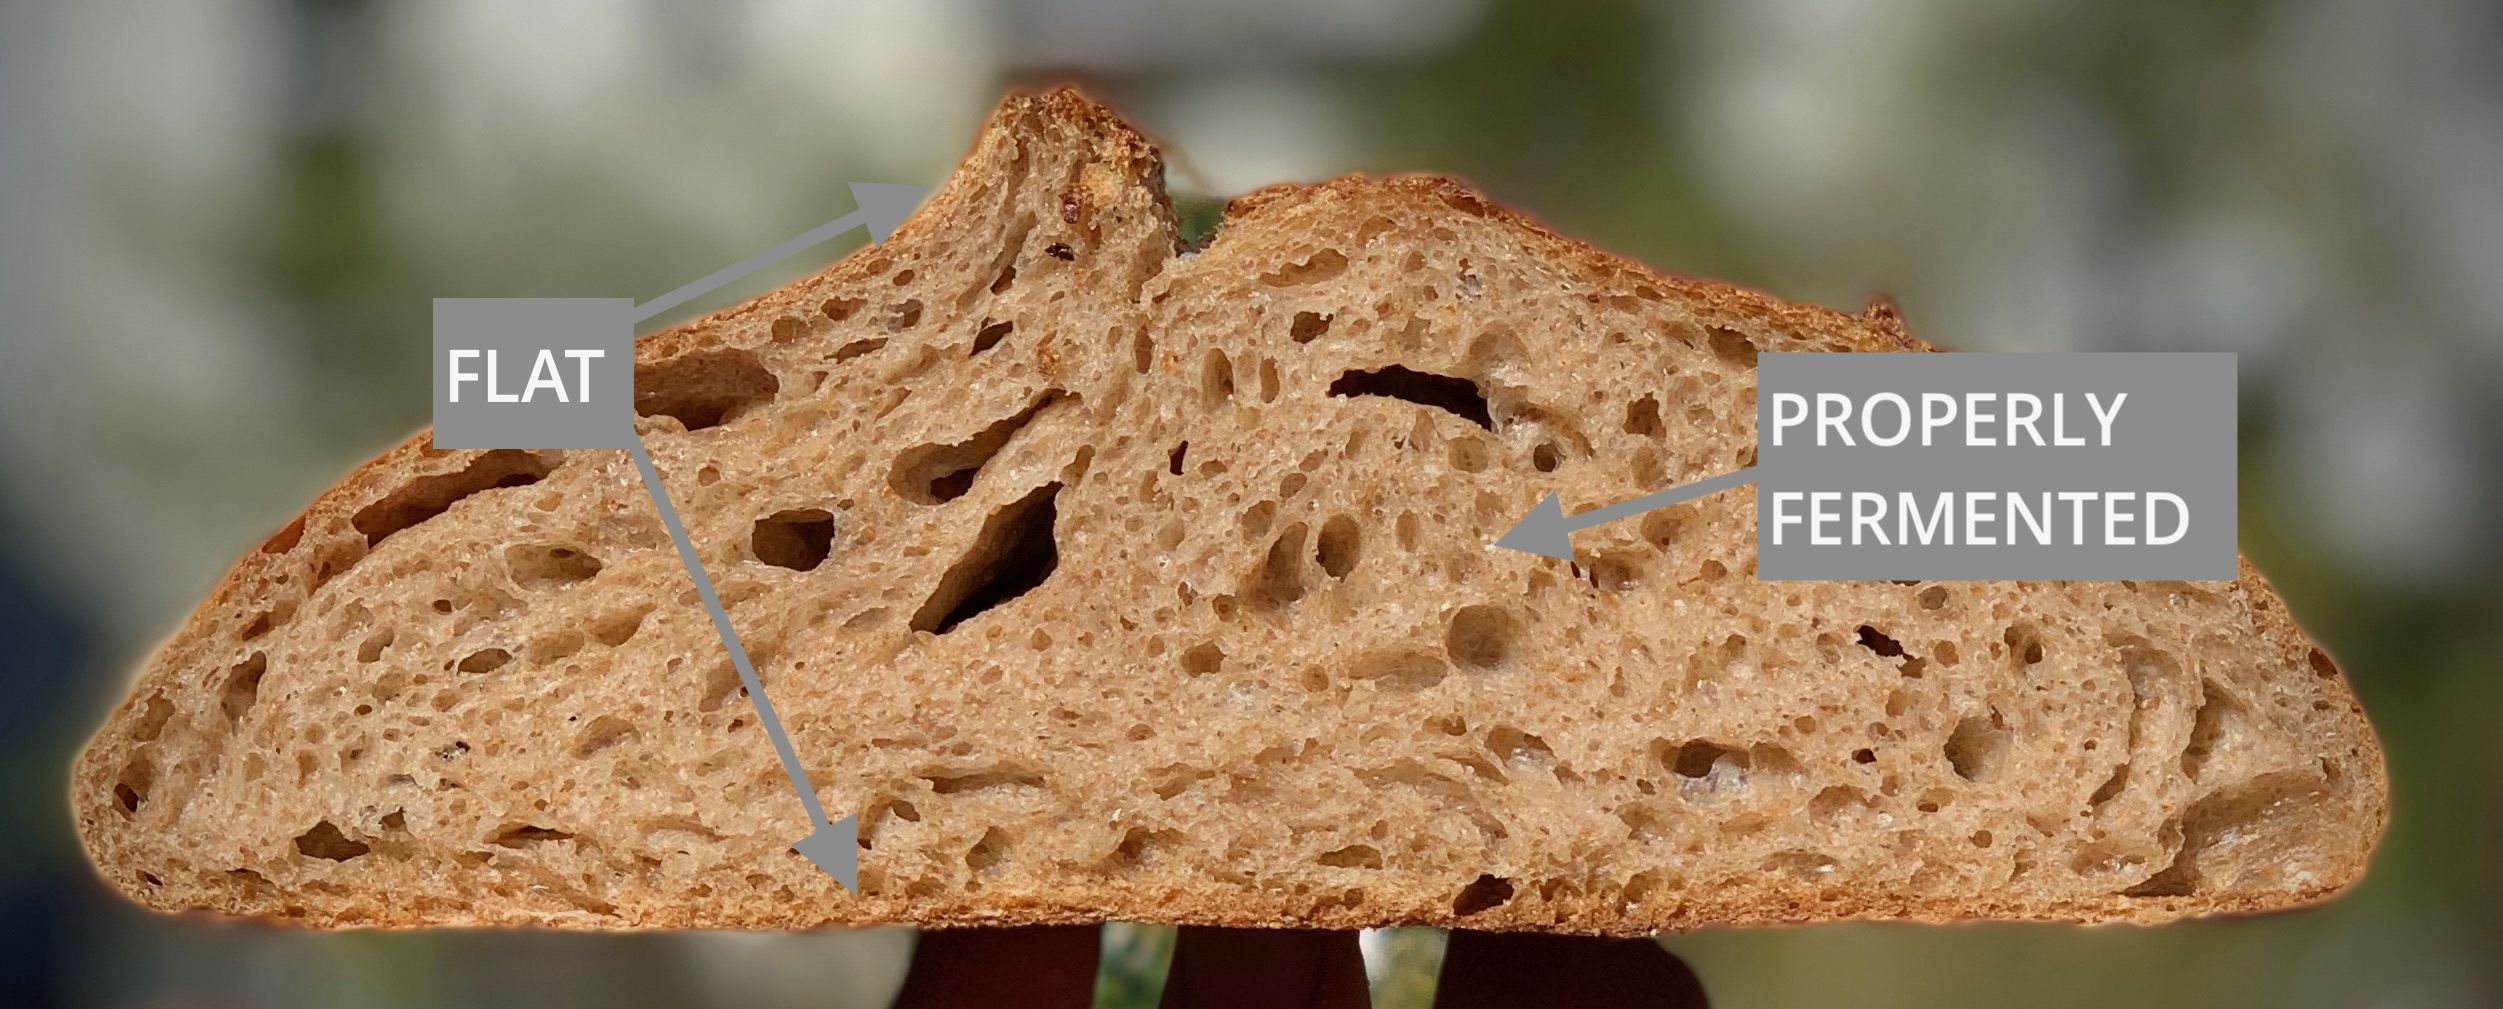
\includegraphics[width=\textwidth]{flat-bread}
  \caption{A very flat bread without enough dough strength.}
  \label{flat-bread}
\end{figure}

When a dough flattens out quite a lot during the baking process chances are
that you did not create enough dough strength. This means your gluten matrix
hasn't been developed properly. Your dough is too extensible and flattens out
mostly rather than springing upwards in the oven. This can also happen if you
proofed your dough for too long. Over time the gluten relaxes and your dough
becomes more and more extensible. You can observe the gluten relaxing behavior
too when making a pizza pie. Directly after shaping your dough balls it's very hard to shape
the pizza pie. If you wait for 30-90 minutes stretching the dough becomes a lot easier.

The easiest way to fix this is probably to knead your dough more at the start. To simplify
things consider using less water for your flour too. This will result in a more elastic dough
right away. This concept is commonly used for no-knead style sourdough.  Alternatively you
can also perform more stretch and folds during the bulk fermentation process. Each
stretch and fold will help to strengthen the gluten matrix and make a more elastic dough.
The last option to fix a dough with too little dough strength is to shape your dough tighter.

\subsection{Baked too hot}

\begin{figure}
  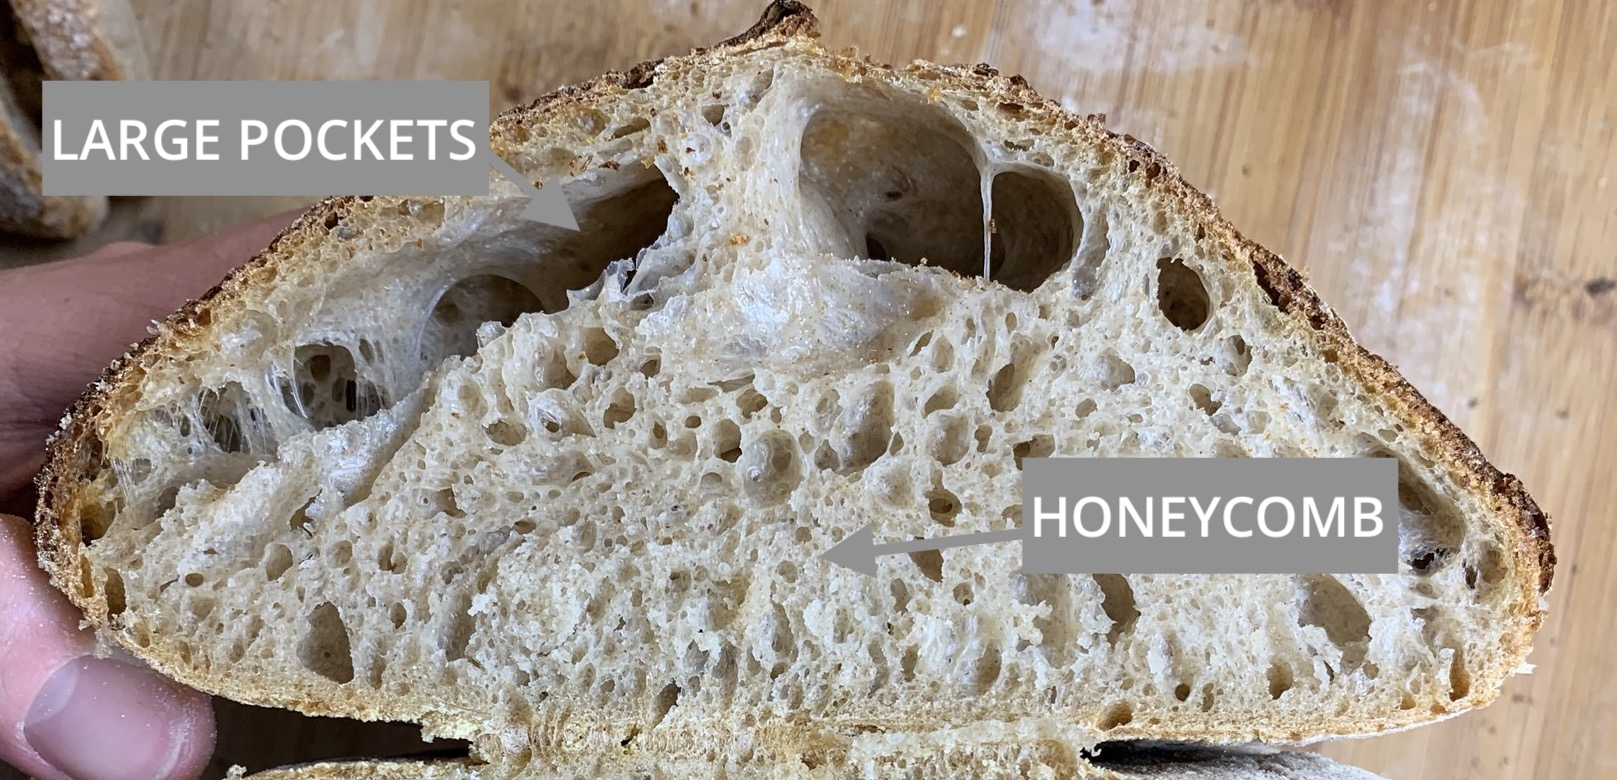
\includegraphics[width=\textwidth]{baked-too-hot-v2}
  \caption{A bread with very large alveoli close to the crust}
  \label{baked-too-hot}
\end{figure}

This is a common mistake that has happened to me a lot. When you bake your dough
at a too hot temperature you block your dough's expansion. The starch gelatinizes
and becomes more and more solid. At around 140°C (284°F) the maillard reaction
starts to completely thicken your bread dough's crust. This is similar to baking
your bread dough without steam. As the internal dough's temperature heats up
more and more water evaporates, gas expands and the dough is being pushed upwards.
Once the dough reaches the crust it can no longer expand. The alveoli merge
into larger structures close to the surface of the dough. By baking too hot
you are not achieving the ear which adds extra flavor. Furthermore your crumb
is not as fluffy as it could be by restricting its expansion capabilities.

If you have an extensible dough with high hydration baking too cold will result
in the dough flattening out quite a lot. The gelatinization of the starch is
essential for the dough to hold it's structure. After conducting several
experiments it seems that my sweet spot for maximum oven spring seems to be
at around 230°C (446°F). Test the temperature of your oven, because in several
cases the displayed temperature might not match the actual temperature of your
oven \cite{too+hot+baking}. Make sure to turn off the fan of your oven. Most
home ovens are designed to vent the steam as fast as possible. If you can not
turn the fan off, consider using a dutch oven.

\subsection{Baked with too little steam}

\begin{figure}[h]
  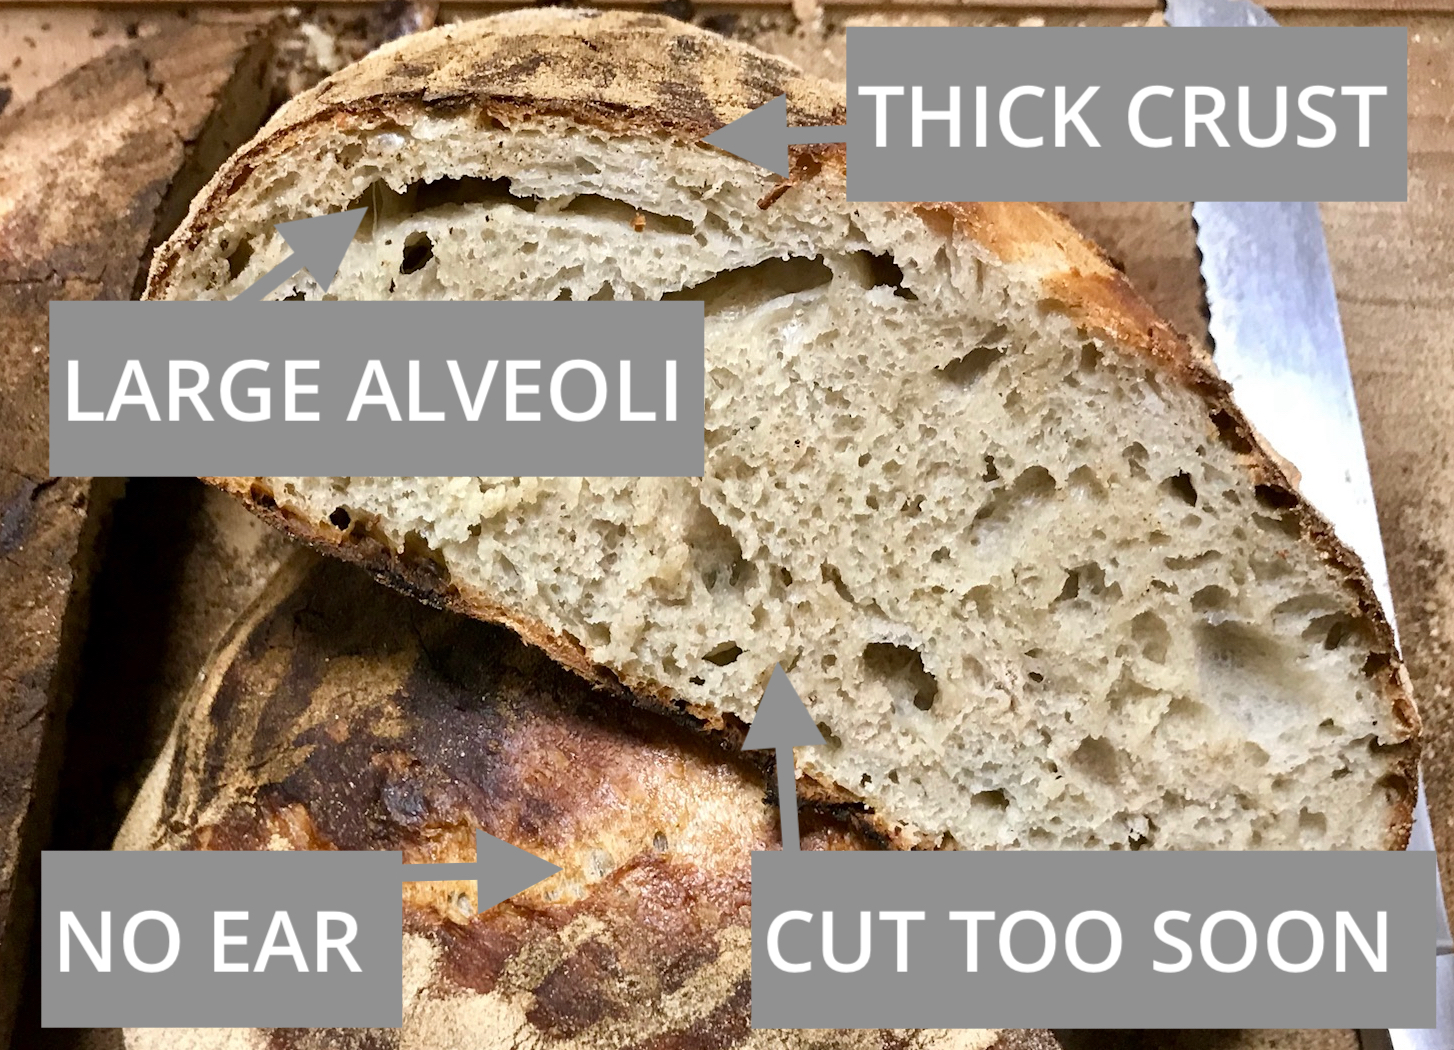
\includegraphics[width=\textwidth]{no-steam}
  \caption{One of my earlier breads that I baked at a friend's place where
  I couldn't steam the dough properly}
  \label{no-steam}
\end{figure}

Similarly to baking too hot when baking without enough steam your dough's crust
forms too quickly. It's hard to spot the difference between the two mistakes.
I typically first ask about the temperature and then about the steaming technique
to determine what might be wrong with the baking process. Too little steam can
typically be spotted by having a thick crust around all around your dough paired
with large alveoli towards the edges.

The steam essentially prevents the maillard reaction from happening too quickly
on your crust. That's why steaming during the first stages of the bake is so important.
The steam keeps the temperature of your crust close to around 100°C (212°F). Achieving steam
can be done by using a dutch oven, an inverted tray and or a bowl of boiling water.
You might also have an oven with a built-in steam functionality. All the methods work,
it depends on what you have at hand. My default go-to method is an inverted
tray on top of my dough, paired with a bowl full of boiling water towards the bottom
of the oven.

\begin{figure}
  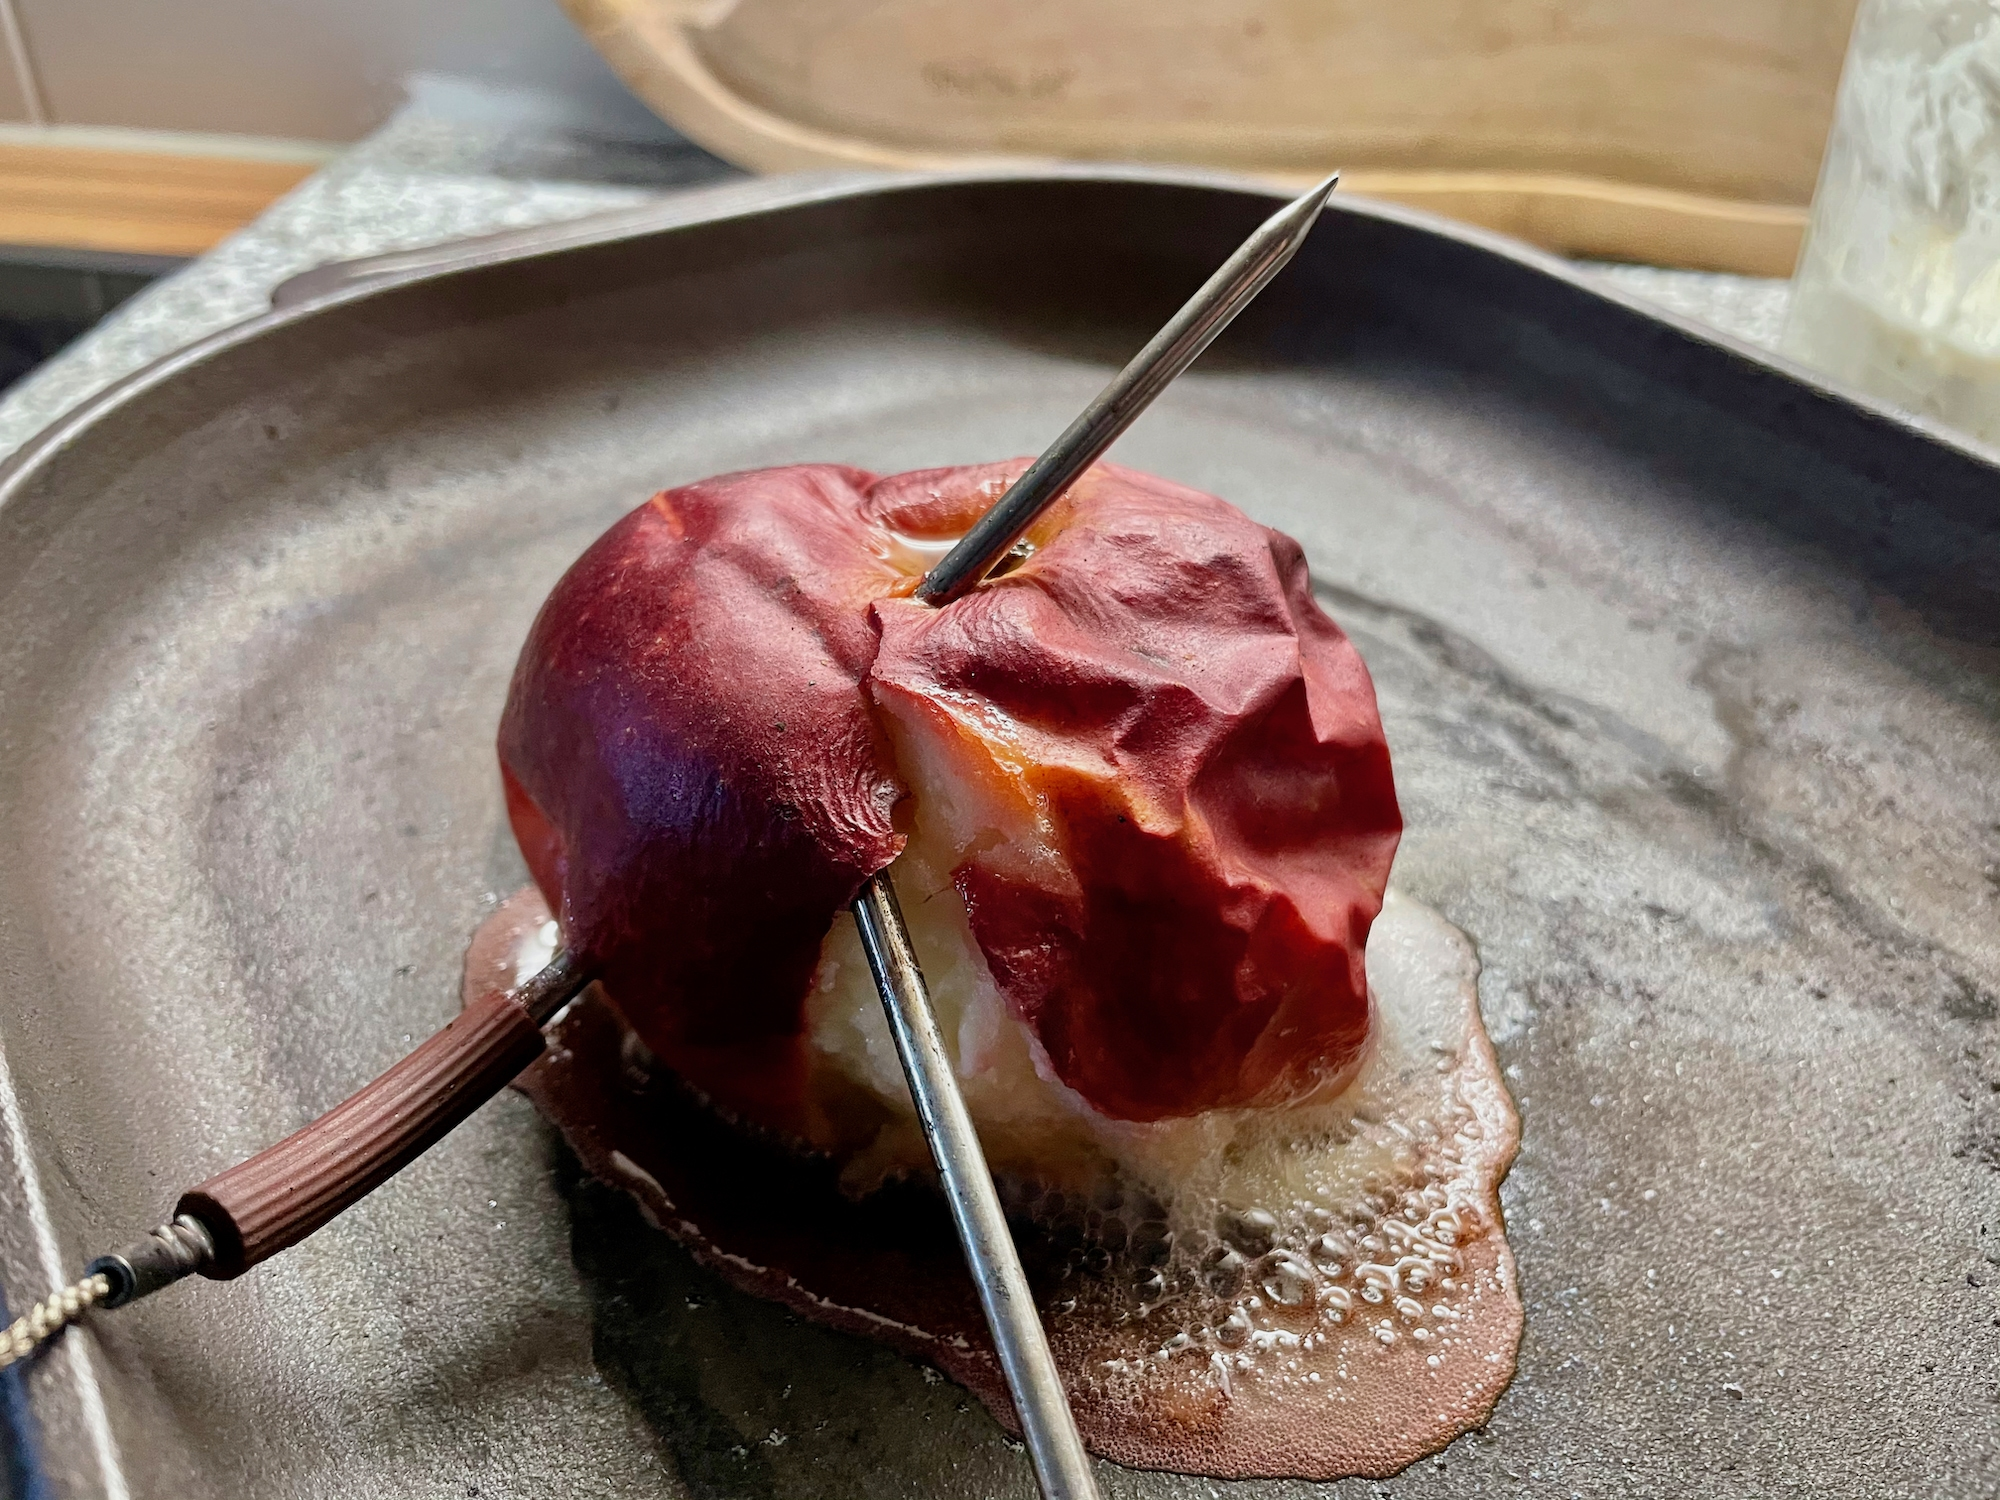
\includegraphics[width=\textwidth]{apple-experiment-temperatures}
  \caption{An apple with 2 probes to measure ambient
  and surface temperatures of several steaming techniques
  in a dutch oven.}
  \label{apple-experiment-temperatures}
\end{figure}

Now there can also be too much steam. For this I tested using a dutch oven paired with large ice
cubes to provide additional steam. The temperature of my dough's surface would directly
jump close to 100°C. The steam contains more energy and can thus through convection
heat up the surface of your dough faster. I tested this by using an apple inside of
a dutch oven. Then I would use a barbecue thermometer with a probe directly at the surface.
I would then change the steaming methods to plot how quickly the temperature
close to the surface of the dough changes. I tried to use an ice cube inside of a preheated
dutch oven, a preheated dutch oven, a preheated dutch oven with spritzes
of water on the apple's surface, a non preheated dutch oven where I would only preheat
the bottom part. The experiment then showed that the ice-cube method would heat up
the surface of the apple a lot quicker. When replicating this with a bread dough
I would achieve less oven spring.

\begin{figure}[h]
  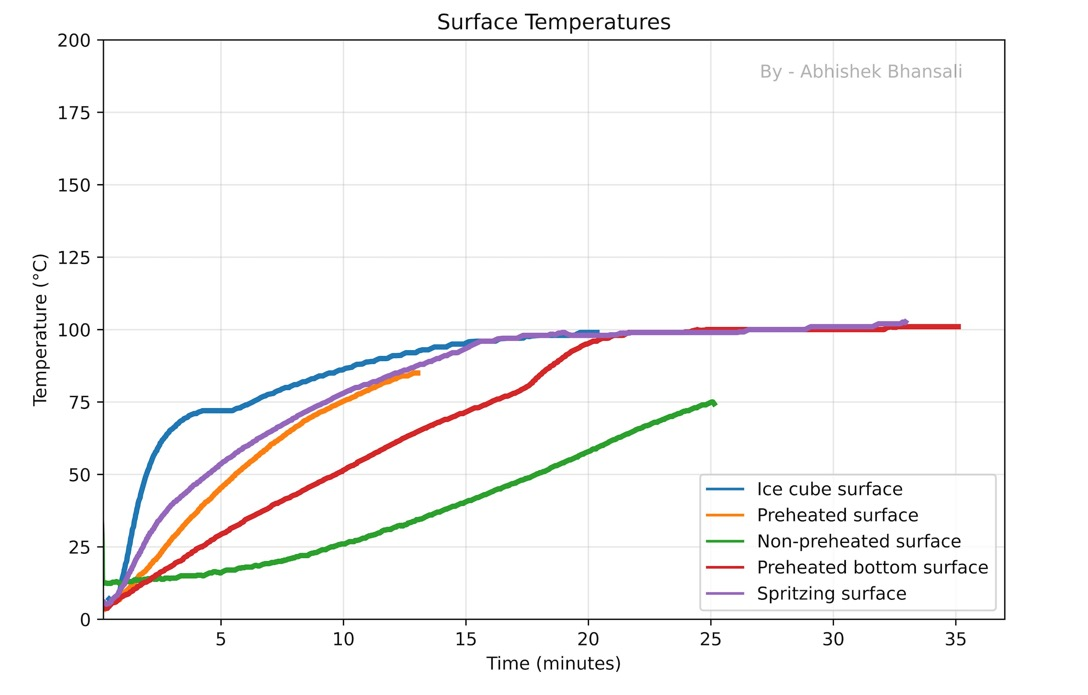
\includegraphics[width=\textwidth]{apple-experiment-surface-temperatures}
  \caption{A chart showing how the temperature of the surface
  of the apple changes with different steaming techniques.}
  \label{apple-experiment-surface-temperatures}
\end{figure}

\begin{figure}[h]
  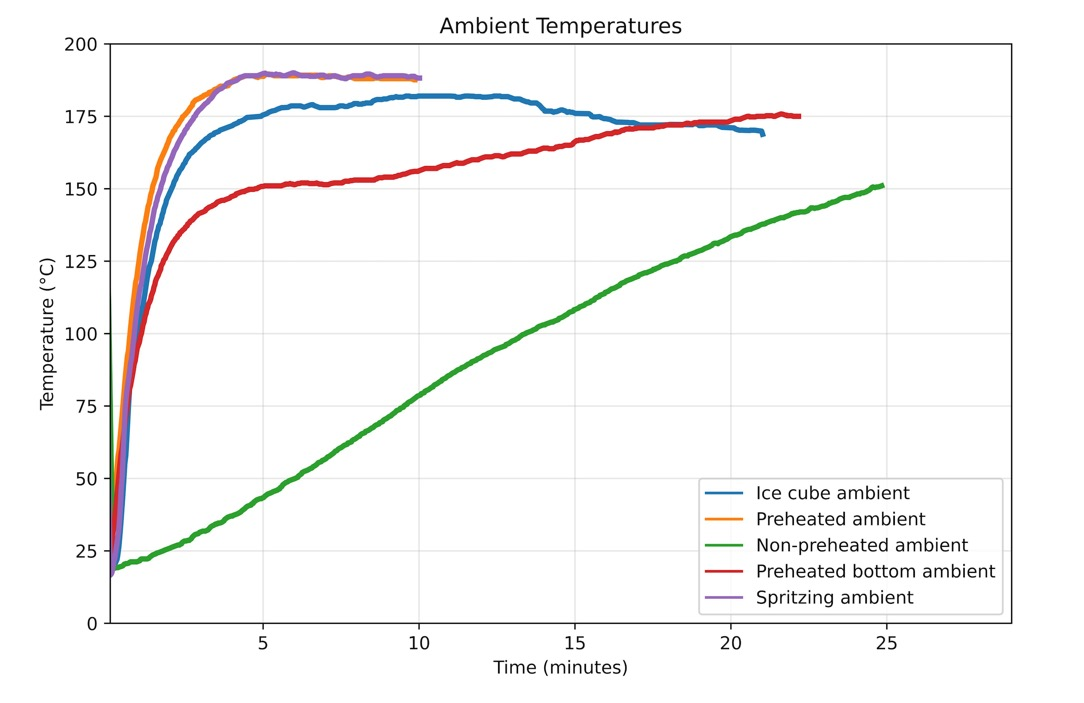
\includegraphics[width=\textwidth]{apple-experiment-ambient-temperatures}
  \caption{This figure shows how the ambient temperatures inside of the
  dutch oven change depending on the steaming technique that is used.}
  \label{apple-experiment-ambient-temperatures}
\end{figure}

Generally though achieving too much steam is relatively challenging. I could only
commit this mistake when using a dutch oven as steaming method paired with relatively
large ice cubes. After talking with other bakers using the same dutch oven, it seems
that mine (around 80g) were 4 times as heavy as the ones other bakers would use (20g)
\section{Baking in the tropics}
\section{My bread stays flat}
\section{I want more tang in my bread}
\section{My bread is too sour}
\section{Fixing a moldy sourdough starter}
\section{My bread flattens out after shaping}
\section{Liquid on top of my starter}
\section{Why does my starter smell like acetone}

\printbibliography


\end{document}